\section{Non-Uniform FFT (NUFFT)}
%=========================================================================================

\begin{frame}{Introduction: Cartesian Sampling (e.g.~FLASH) \footnote{Haase A, Frahm J, Matthaei D, Hanicke W, Merboldt KD. FLASH imaging. Rapid NMR imaging using low flip-angle pulses. \textit{J Magn Reson} (1986).}}

	\begin{columns}
		\begin{column}{0.45\textwidth}
			\begin{figure}
				\includegraphics[width=\columnwidth]{fig/mri-seq-ge-cart.png}
			\end{figure}
		\end{column}

		\begin{column}{0.35\textwidth}
			\begin{figure}
				\includegraphics[width=\columnwidth]{fig/mri-trj-cartes.png}
			\end{figure}
		\end{column}
	\end{columns}
\end{frame}


\begin{frame}{Introduction: Fast Fourier Transform}

	\begin{equation}
		s(k_x, k_y) = \int \rho(x, y) \cdot e^{-i (k_x \cdot x + k_y \cdot y)} \text{d}x \text{d}y
	\end{equation}

	\begin{figure}
		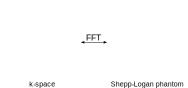
\includegraphics[width=0.7\textwidth]{fig/fft.png}
	\end{figure}

\end{frame}


\begin{frame}{Non-Cartesian Sampling (e.g.~ Radial \footnote{Lauterbur PC. Image formation by induced local interactions: Examples employing nuclear magnetic resonance. \textit{Nature} (1973).} and Spiral \footnote{Nishimura DG, Irarrazabal P, Meyer C. A velocity k-space analysis of flow effects in echo-planar and spiral imaging. \textit{Magn Reson Med} (1995).})}

    \begin{columns}
		\begin{column}{0.35\textwidth}
			\centering
			Radial
			\begin{figure}
				\includegraphics[width=\columnwidth]{fig/mri-trj-radial.png}
			\end{figure}
		\end{column}

		\begin{column}{0.35\textwidth}
			\centering
			Spiral
			\begin{figure}
				\includegraphics[width=\columnwidth]{fig/mri-trj-spiral.png}
			\end{figure}
		\end{column}
	\end{columns}
\end{frame}


\begin{frame}
    \begin{figure}
        \centering
        \includegraphics[page=3, width=0.8\textwidth]{fig/noncartesian_mri_overview.pdf}
    \end{figure}
    \blfootnote{Courtesy: Dr.~Frank Ong @ UC Berkeley}
\end{frame}


\begin{frame}{Image Reconstruction of Non-Cartesian Data Requires NUFFT}
	NUFFT: Non-Uniform FFT \footnote{OSulllivan J. A fast sinc function gridding algorithm for Fourier inversion in computed tomography. \textit{IEEE Trans Med Imaging} (1985).}
	$^,$ \footnote{Jackson J, Meyer CH, Nishimura DG, Macovski A. Selection of a convolution function for Fourier inversion using gridding. \textit{IEEE Trans Med Imaging} (1991).}
	$^,$ \footnote{Fessler JA, Sutton BP. Nonuniform fast Fourier transforms using min-max interpolation. \textit{IEEE Trans Med Imaging} (2003).}
    \vspace{1em}
	\begin{enumerate}
		\item Density compensation
		\item Gridding: Convolution with the Kaiser-Bessel window
		\item Deapodization \& Inverse FFT
	\end{enumerate}
\end{frame}


\begin{frame}[fragile]{NUFFT Step 1: Density Compensation}

    \begin{itemize}
        \item Non-Cartesian samples are usually not uniformly acquired in $k$-space.
        \item e.g.~In radial sampling, the central $k$-space points are more densely acquired than peripheral $k$-space points.
        \item Analytical density compensation function (DCF) in radial sampling. \\
        \vspace{1em}
        Given $\mathrm{ktrj} = k_x + 1i * k_y$, \\
        \begin{equation}
        	\mathrm{DCF} = \sqrt{k_x^2 + k_y^2}
        \end{equation}
    \end{itemize}

\end{frame}


\begin{frame}{DCF in Radial Sampling}

    \begin{columns}
	\begin{column}{0.35\textwidth}
		\centering
		Radial
		\begin{figure}
			\includegraphics[width=\columnwidth]{fig/mri-trj-radial.png}
		\end{figure}
	\end{column}

	\begin{column}{0.35\textwidth}
		\centering
		DCF
		\begin{figure}
			\includegraphics[width=\columnwidth]{fig/dcf.png}
		\end{figure}
	\end{column}
	\end{columns}

\end{frame}


\begin{frame}{NUFFT Step 2: Gridding (Interpolation) with the Kaiser-Bessel Window}

    \begin{columns}
	\begin{column}{0.65\textwidth}
		\centering
		Interpolation  \footnote{\url{https://users.fmrib.ox.ac.uk/~karla/reading_group/lecture_notes/AdvRecon_Pauly_read.pdf}}
		\begin{figure}
			\includegraphics[width=\columnwidth]{fig/interp.png}
		\end{figure}
	\end{column}

	\begin{column}{0.30\textwidth}
		\centering
		Kaiser-Bessel Window
		\begin{figure}
			\includegraphics[width=\columnwidth]{fig/kb.png}
		\end{figure}
	\end{column}
	\end{columns}

\end{frame}


\begin{frame}{NUFFT Step 3: Deapodization}

	\begin{itemize}
		\item The gridded signal on Cartesian grids can be written as the convolution between the non-Cartesian signal and the Kaiser-Bessel window,
		\begin{equation}
			s_\mathrm{Cart} = s_\mathrm{non-Cart} \circledast W_\mathrm{kb}
		\end{equation}

		\vspace{1em}

		\item with FFT, it becomes
		\begin{equation}
			\mathcal{F} \{s_\mathrm{Cart} \} = \mathcal{F} \{ s_\mathrm{non-Cart} \} \cdot \mathcal{F} \{ W_\mathrm{kb} \}
		\end{equation}

		\vspace{1em}

		\item Then deapodization is
		\begin{equation}
			I = \mathcal{F} \{s_\mathrm{Cart} \} ./ \mathcal{F} \{ W_\mathrm{kb} \}
		\end{equation}

	\end{itemize}

\end{frame}


\begin{frame}{NUFFT Implementations}
    \begin{enumerate}
        \item Python / PyTorch -
        \vspace{1em}
        \begin{itemize}
            \item sigpy: \url{https://github.com/mikgroup/sigpy}
            \vspace{0.5em}
            \item torchkbnufft: \url{https://github.com/mmuckley/torchkbnufft}
        \end{itemize}

        \vspace{2em}
        \item C -
        \vspace{1em}
        \begin{itemize}
            \item Gridding Functions: \url{http://mrsrl.stanford.edu/~brian/gridding/}
            \vspace{0.5em}
            \item BART: \url{https://github.com/mrirecon/bart}
        \end{itemize}
    \end{enumerate}
\end{frame}


\begin{frame}{NUFFT Exercises}
	\begin{itemize}
		\item Double "num\_samples" in the function "make\_adc"
		\vspace{1em}
        \item Reduce "Nphase", what undersampling artifacts do you see?
        \vspace{1em}
		\item What artifacts do you see in the presence of gradient delays?
		\vspace{1em}
        \item How would you correct for gradient delays in reality?
		\vspace{1em}
        \item What if the density compensation function is unknown?
	\end{itemize}
\end{frame}
